\documentclass[11pt,a4paper]{article}
%\usepackage[toc,page]{appendix}
\usepackage{graphicx}
\usepackage[a4paper]{geometry}
\usepackage{xcolor}
\usepackage{fancyhdr}
\usepackage{float}
\usepackage{setspace}
\usepackage[absolute]{textpos}
\usepackage{epstopdf}
%\usepackage[]{mcode} 	% To include matlab code
\usepackage{capt-of}
\usepackage{enumerate}
\usepackage{lastpage}
\usepackage{booktabs}
\usepackage{longtable}
\usepackage{array}
\renewcommand{\arraystretch}{1.5}

\usepackage[english]{babel}
\usepackage[utf8]{inputenc}
\usepackage{amsmath}
\usepackage{amsfonts}
\usepackage{graphicx}
\usepackage[colorinlistoftodos]{todonotes}
\usepackage{algorithm}
\usepackage{algpseudocode}

\usepackage{amsmath}
\usepackage{algorithm}
%\usepackage[noend]{algpseudocode}
\makeatletter
\def\BState{\State\hskip-\ALG@thistlm}
\makeatother

\usepackage{amsmath}
\usepackage{amsfonts}
\usepackage{amssymb}
\usepackage{eurosym}

% Header
\setlength{\headheight}{30pt}
\newgeometry{top=2.5cm, bottom = 1.5cm, left=2cm, right=2cm}
\pagestyle{fancy} 
\lhead{\includegraphics[height=0.8cm]{figures/{tue_logo}.png}}
%\lfoot{Group 4 - ``CASE"-HENK}
\cfoot{~}
\rfoot{Page \thepage ~of \pageref{LastPage}}

\usepackage{cleveref}
% Change cleveref reference eq. to equation same for figure
\crefname{equation}{equation}{equations}
\crefname{figure}{figure}{figures}
\crefname{table}{table}{tables}

% Change Section numbering to Problem 1
%\renewcommand{\thesection}{Problem \arabic{section}.}

\begin{document}
%\begin{titlepage}
%\vspace*{100pt}
%\begin{figure}
%\centering
%\includegraphics[width=0.5\textwidth]{figures/TUelogozondertekst}
%\end{figure}
%\begin{center}
%{ \huge \bfseries 4AT100 Automotive Systems Engineering Project\\[0.4cm] }
%\textsc{\Large Concept Project Plan}\\[0.5cm]
%
%\end{center}
%
%\vfill
%
%\renewcommand{\arraystretch}{1}
%
%\begin{flushleft} \large
%\begin{tabular}{l}
%Project Coordinators:\\
%Dr.Ir. A. van de Mortel-Fronczak (Asia) \\
%Dr.Ir. I. Barosan (Ion) \\
%\end{tabular}
%\end{flushleft}
%
%\begin{flushleft} \large
%\begin{tabular}{l l l l}
%Tutor: & & & \\
%L. Kefalidis (Lazaros) & & & \\
%& & & \\
%Authors:\hspace{30mm} 	& \hspace{35mm}	& \hspace{55mm} 	    		& 			\\
%S. Forno (Simone) 		& ​0978942		& T. de Mor\'ee (Tim)			& 0944052 	\\
%R.M.A. Goris (Rob) 		& 0808822		& T.M.A. van de Wiel (Thijs)	​& 0824530 	\\
%B.S. Haarsma (Bouke) 	& 0751757​		& H. Wils (Hielke) 				& 0807014 	\\
%\end{tabular}
%\end{flushleft}
%
%\begin{flushleft} \large
%\begin{tabular}{l}
%MSc. Programme Automotive Technology \\
%Eindhoven University of Technology \\
%\end{tabular}
%\end{flushleft}
%
%\begin{flushleft} \large
%\begin{tabular}{l}
%\today \hspace{8.4cm} Group 4 ``CASE"-HENK \\
%\end{tabular}
%\end{flushleft}
%
%\renewcommand{\arraystretch}{1.5}
%
%\end{titlepage}

\newgeometry{top=2.5cm, bottom = 3cm, left=2cm, right=2cm}

%\newpage
%
%\setcounter{tocdepth}{2}
%
%\tableofcontents
%\newpage


%------------------------------------------------

\section{Remote Localization study} \label{sec:res}

An example of Husky link and joint, see Figure below.

\begin{figure}[!h]
    \centering
    \begin{minipage}{.5\textwidth}
        \centering
        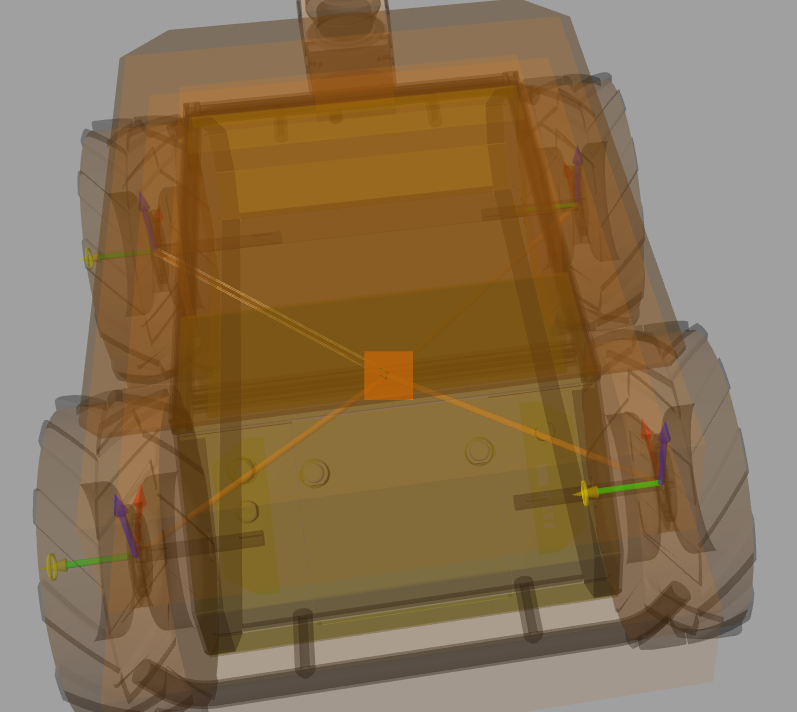
\includegraphics[width=0.7\linewidth, height=0.2\textheight]{figures/husky_joint}
        \caption{Husky joint}
        \label{fig:}
    \end{minipage}%
    \begin{minipage}{0.5\textwidth}
        \centering
        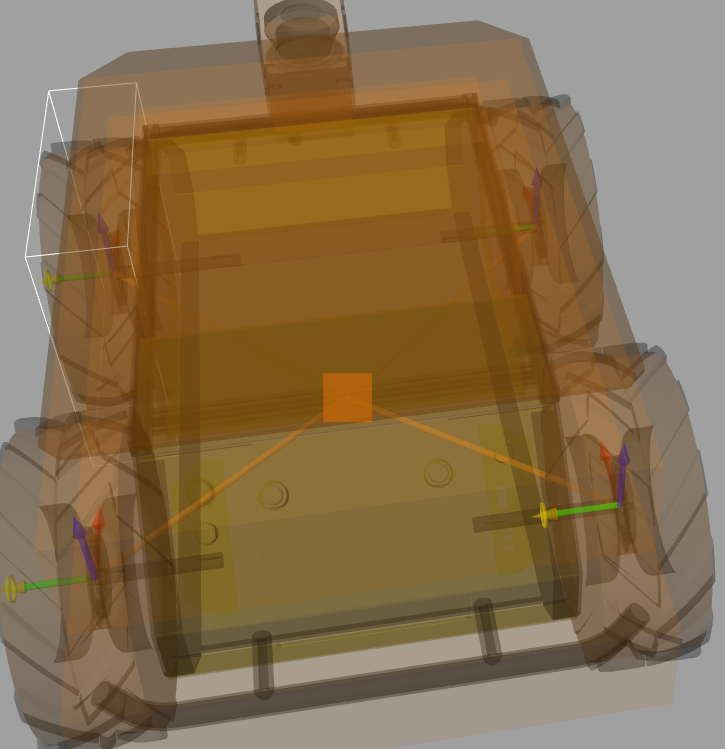
\includegraphics[width=0.7\linewidth, height=0.2\textheight]{figures/husky_link}
        \caption{Husky link}
        \label{fig:}
    \end{minipage}
 \end{figure}

\textbf{Main question} is how are links and joints and other parameters from Gazebo node read? There should be a sort of .cpp file reading those params. The package that handles this is the \textbf{gazebo-ros-pkg}, further documentation is found here: http://wiki.ros.org/ros{\_}control. \\

\begin{figure}[H]
	\center
	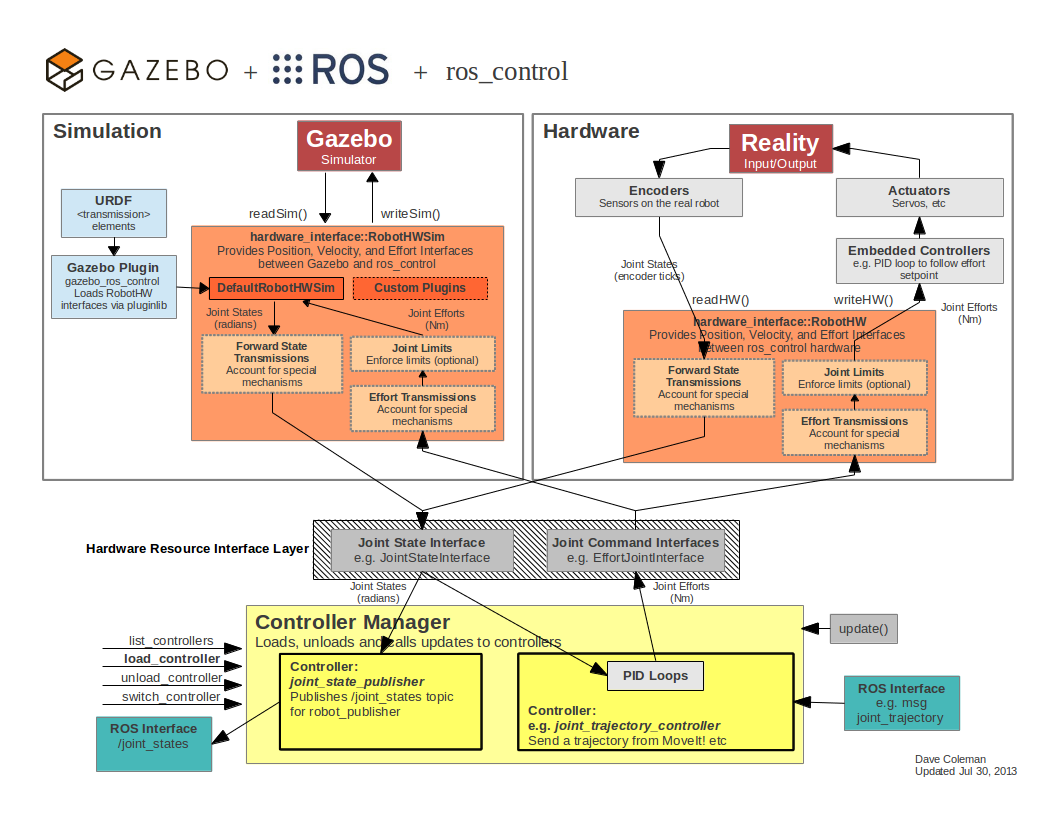
\includegraphics[width=.9\textwidth]{figures/gazebo_ros_transmission.png}
	\caption{gazebo ros transmission}
	\label{fig:ros_control}
\end{figure}

Figure \ref{fig:ros_control} shows the schematics for gazebo{\_}ros control interfaces, for controlling the robot. The final output are joint states published in the /joint-state topic. Even if not specifically inherent with localization tags, this example shows how Gazebo plugins work and how the \textbf{Gazebo sim} exposes with interfaces. \\
For the specific case, the gazebo plugin is under the file \textbf{description.gazebo.xacro} and the transmission tags read by the Plugin under \textbf{wheel.urdf.xacro}. The cpp files actually reading URDF. \\
\textbf{Question}: How is for example the \textbf{/scan} topic exposed out from the Gazebo simulation? Which .cpp file does expose the URDF code into a topic? This is done by the plugin .cpp file under the \textbf{gazebo-ros-pkgs/gazebo-plugins}. Ones the code is compiled a $shared object-*so$ file is produced and hence the plugin is active, ready to be added into the robot \textbf{xacro URDF file with <gazebo> tag}. \\
See below pictures for explanation:

\begin{figure}[!h]
    \centering
    \begin{minipage}{.5\textwidth}
        \centering
        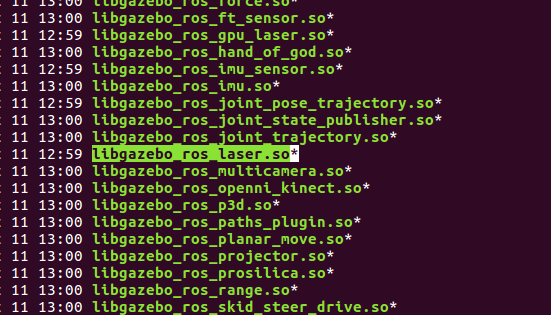
\includegraphics[width=0.8\linewidth, height=0.2\textheight]{figures/laser_plugin}
        \caption{The .so* file}
        \label{fig:}
    \end{minipage}%
    \begin{minipage}{0.5\textwidth}
        \centering
        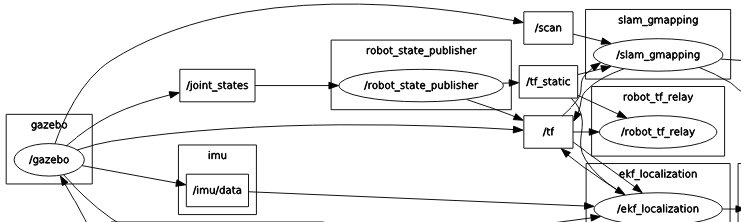
\includegraphics[width=1\linewidth, height=0.15\textheight]{figures/scan_topic}
        \caption{The scan topic is visible only when some node is subscribing to it; however if the simulation is run from Gazebo only (roslaunch husky{\_}gazebo husky{\_}fabrichalle) the scan is already into the topic list. This means that the plugin already activates it.}
        \label{fig:}
    \end{minipage}
 \end{figure}

\begin{figure}[H]
	\center
	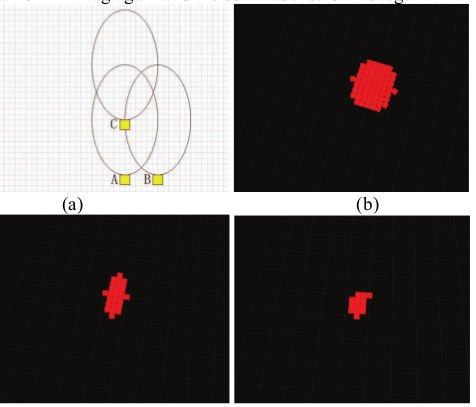
\includegraphics[width=.4\textwidth]{figures/tags.png}
	\caption{Example of triangulation to estimate the pose of an RFID tag}
	\label{fig:tag}
\end{figure}


\subsection{Reading paper of RFID tags}
[2]: See the reference number 3 of Tesoriero for a general RFID tags overview \\
Use RFID passive tags as in the approach of paper [3] with a similar client-server architecture. In this paper they propose a combination of SLAM and RFID tags to retrive the locations of objects, attaching on them the radio-frequency tags only. Main goal is therefore extimating the objects position.\\
\textbf{System overview and approach} The approach is divided in different software levels, the 1st to be the object identification and rough estimation of its position (RFID retrieves the object ID, color,shape, etc..), the 2nd SLAM gives the robot`s pose + RFID reader detect the object tag. Given the infos of the RFID to the laser, the laser device can then recognize the object, its area and position. As soon as an object carrying a tag is detected, the robot position is stored (from SLAM) and estimate the existing area of the object is calculate. By measuring the same tag in different positions, the RFID tag position can be estimated with a triangulation algorithm (See Figure \ref{fig:tag}). This is basically overlapping of single maps in different times. When A and B are detected, the possible area is the intersection of the 2, but when a new one C is detected, the area schrinks to a smaller value. This smaller area is needed for roughly saying to the robot where to look. Then a vision algorithm is used to get the proper info semantics (ID, ...). \\
Even if interesting articles, this would not solve the main goal of localization in my case. It would be interesting to see the coin on the other side. Given I know the object, I should get the robot position. The approach in the paper [3] looks more similar to this idea. \\
However the key idea behind this paper may not be useless for me. In \textbf{[4]} the actual estimation of RFID tags can be used to build an $RFID$ specific map, in which a robot can be localized. \\



[3]: In this article we propose the use of a cheap and reliable technology as RFID to develop a passive RFID-based indoor location system that is able to accurately locate autonomous entities. Passive RFID tags do not have an internal battery and are energized from antenna readers, as soon as the reader approaches the tag. Main KPI of Indoor systems are $accuracy$, hence how much it deviated from the real trajectory (\textbf{odom filtered for us}) and $environmental factors$, such as the positioning of the tags into the environment should not affect the localization performance. \\
\textbf{An overview of indoor localization systems}: 
\begin{enumerate}
\item Wifii have low accuracy (3-5 m), may be affected from strong signal reflection that further reduce the performance
\item Low accuracy, frequency communication between devices can take long time, no possibility to use RSSI signal strenght to measure the distance
\item Ultrasound devices can have good accuracy if the deployment of the tags is dense enough throughout the space
\item RFID used in this paper are passive, positioned into sensing surfaces. Each of the surfaces is divided into $location units$, each of which has one specific ID. By knowign the unique ID, a system is able to localize into an environment. To get those IDs the robot must be equipped with a passive ID reader (mmhhhh \textbf{In Gazebo can't we just send the ID outside the simulation and let it read by the robot?}). Indeed we do not focus on the communication between the single ID and the map itself (the architecture is based on client-server mode), but we are happy as soon as the ID is sent out from the simulation.
\item Evaluating the positioning system. There are two configuration parameters that are important to be taken into account to get a reasonable performance of location
systems in RFID. These are the reading and timeout times. 
\end{enumerate}

[4]: This paper present a way to localize RFID readers into an environment. The generated maps with RFID tags are used to localize the robot or better to improve the robot localization within the map. \\
The robot needs to be equipped with an RFID antenna, in order to read radio frequency signals from static world tags. \textbf{Detection range is around 6 meters}. The antennas are used to estimate the position of tags, and here the proper \textbf{sensor model} should be defined (like for the laser the laser beam model). The estimation of location tags uses antenna on the robot and the map mapped with laser data.\\
RFID can be used to actually map an environment, like the method proposed by Kanton and Singh, which uses \textbf{active beacons} to calculate \textbf{distance, based on the time required to receive the response of a tag - in this I have to think that beacons are triggered by a sort of service call and the response time from the service call determines the time for distance - mmhh this makes sense indeed}, the position of the tags have to be known accurately - here we can place the hypothesis that we localize given known poses of tags, hence we just perform \textbf{localization} and not mapping. \\
In this paper they want to first estimate the positions of tags and then localize. To do so, the posterior should be calculated: 
\begin{equation}
p(x|z_{1:t},r_{1:t}) = p(z_t|x,r_t)p(x|z_{1:t-1},r_{1:t-1}) \label{eq:1}
\end{equation}

The measurement model (likelihood model) is the term $p(z_t|x,r_t)$, which has been determined empirically in this paper (no formulas). The environment is first mapped, then Eq. \ref{eq:1} is run to estimate the positions of tags. It uses a sort of particle filter to first choose random positions, stores each posterior $p(x|z_{1:t},r_{1:t})$ with a numerical value, then when tag is detected the posterior is updated (assigning weights???) based on \ref{eq:1}, using the antenna sensor model. \\

Anyway what is interesting for us is \textbf{Section V: Localization with RFID tags}, given the tag poses are known (or posterior $p(x|z_1:t,r_1:t)$). Defining the likelihood of an observation $y$, given we know the robot location $l$. According to this law:
\begin{equation}
p(y|l) = \sum_{x} p(y|x,l)p(x|z_1:t,r_1:t) \label{eq:2}
\end{equation}

This equation represents a corresponding term for the \textbf{Localization}, like $p(z_t|x,r_t)$, hence this is the observation model.
The second term is \textbf{known}, the first term corresponds to the \textbf{relative sensor model}, hence $p(z_t|x,r_t)$. The assumption is here that the likelihood sensor model \textbf{ONLY} depends on the relative offset betweem the tag pose $x$ and the robot antenna $r$. For this case the offset is computed from the difference between the robot pose $l$ and the tag $x$. To calculate \ref{eq:2} we sum up, or integrate this term over all the posterior probability of the tag`s location $x$. \\
The \textbf{final goal} is however to estimate the robot pose. This resamble the left part of Equation 3:

\begin{figure}[h]
	\center
	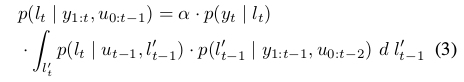
\includegraphics[width=.6\textwidth]{figures/eq.png}
\end{figure}

The first part of the right end side of the equation is the probability that the robot is at position $l_t$ given the previous poses and the commands $u_t$, odometry. \textbf{This can be computed using the motion model, see file SelfLocalizer; applying Amcl with Pf like the .cpp file can be an idea}. The quantity $p(y_t|l_t)$ is already computed in equation \ref{eq:2}. \\
\textbf{How is the posterior in equation 3 computed?} \\
They use Amcl with PF, each particles is a state vector with the pose $l$ and the weight $w$, as usual for the Amlc particle filter. Prediction and correction step are as follows: 

\begin{itemize}
\item \textbf{prediction step} apply each sample using weight (\textbf{mhhhh do samples already have a weight in the prediction?}) and motion model (same as Amcl)
\item \textbf{correction step} Assign a new $w$ according to observation $p(y_t|l_t)$. \textbf{IMPORTANT}: We place samples not randomly in the environment, but only in the RFID sensor range.
\end{itemize}





\subsection{References}
\begin{enumerate}
\item From $http://gazebosim.org/tutorials?tut=plugins{\_}hello{\_}worldcat=write{\_}plugin$ - Use a Sensor plugin to acquire sensor information and control sensor properties.
\item RFID paper: ROS-based Object Localization Using RFID and Laser Scan, Shujun Gong, Huifen Liu, Ying Hu, Jianwei Zhang.
\item Improving location awareness in indoor spaces using RFID technology, Tesoriero
\item Mapping and Localization with RFID Technology, Dirk Hähnel Wolfram Burgard Dieter Fox Ken Fishkin Matthai Philipose.
\item I might want to see, reference from paper [4]: [9] George A Kantor and Sanjiv Singh. Preliminary results in range-only localization and mapping, [14] Sanjiv Singh, George Kantor, and Dennis Strelow. Recent results in extensions to simultaneous localization and mapping, [16] T. Tsukiyama. Navigation system for mobile robots using RFID tags. Those paper present localization using RFID tags with \textbf{known position, so localization upon known position is performed}.
\end{enumerate}



\end{document}


% == TABLE ==
%begin{table}[h!]
 % \centering
  %\caption{Caption for the table.}
 % \label{tab:table1}
 % \begin{tabular}{ccc}
 %   \toprule
  %  Some & actual & content\\
   % \midrule
   % prettifies & the & content\\
   % as & well & as\\
  %  using & the & booktabs package\\
  %   \bottomrule
  %\end{tabular}
%\end{table}


% === ALGORITHM == 

{\_}

\iffalse % multi-comment tool
\begin{algorithm}[!h]
   \caption{Kirsch, Rohig algorithm}
    \begin{algorithmic}[1]
    	\State $St-1 = St$
        \For{$i = 1$ to $N$} \Comment{With N the number of particles in the filter set by maxparticle parameter}
            \State $Spread $ $particles$ $in$ $the$ $anchorbox$ $with$ $equations$ $1)$ $and$ $2)$ $of$ $[3]$ \Comment{This step is called $Global$ $Localization$}
            
            \State $xt[n] = p(xt|xt-1,ut)$ \Comment{Motion update - sample the particles from the motion update of the robot and move forward to estimate the error model functions}
            
        	\State $wt[n] = p(dnanoLOC|si)*p(dlaser|si)$ \Comment{Measurement update - si are the particles set with i the i-th index}
        	\State $St = St + <xt,wt>$ \Comment{add the state and weight to the total state space}
        	
        	\State $Perform$ $resampling$
        \EndFor
    \State $Return$ $St$

\end{algorithmic}
\end{algorithm}
\fi


\iffalse

\begin{figure}[!htb]
    \centering
    \begin{minipage}{.5\textwidth}
        \centering
        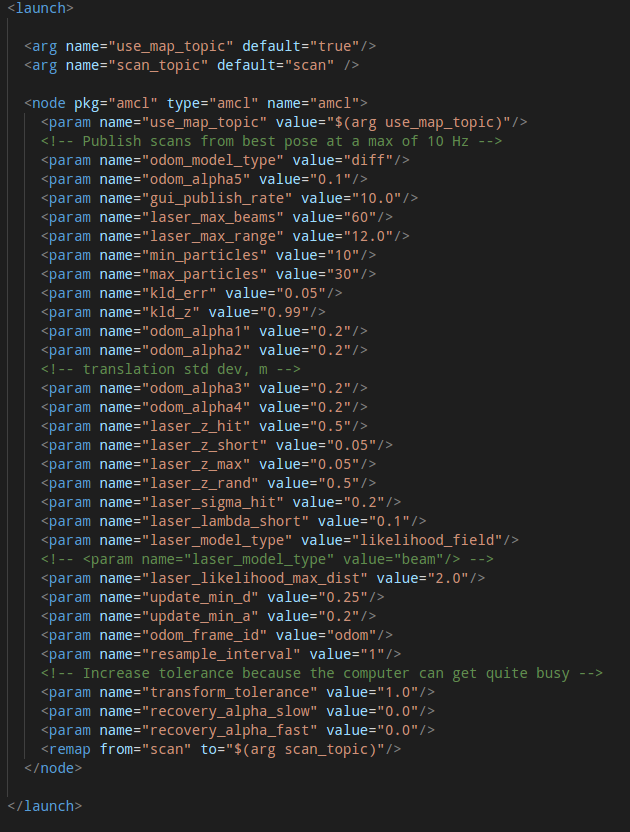
\includegraphics[width=0.7\linewidth, height=0.2\textheight]{figures/amcl_param}
        \caption{The $amcl$ tunable parameters}
        \label{fig:amcl_param}
    \end{minipage}%
    \begin{minipage}{0.5\textwidth}
        \centering
        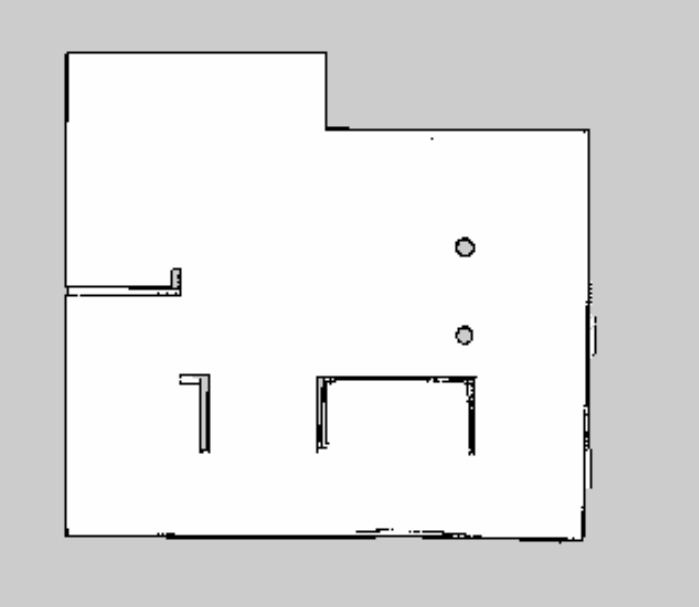
\includegraphics[width=0.7\linewidth, height=0.2\textheight]{figures/my_amcl_gmapping}
        \caption{Result of the Gmapping for the simple indoor environment}
        \label{fig:myamcl_map}
    \end{minipage}
 \end{figure}
 
 
 
\begin{figure}[!htb]
	\center
	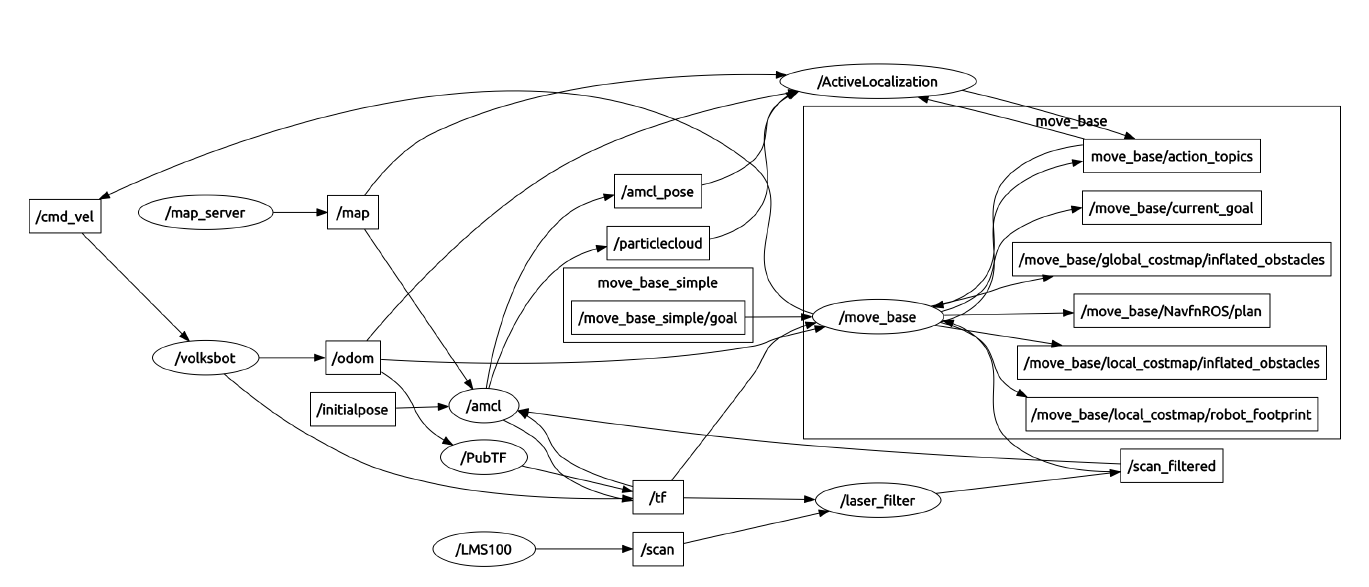
\includegraphics[width=1\textwidth]{figures/active_localization_node.png}
	\caption{An example of an active localization node}
	\label{fig:active_locnode}
\end{figure}


% underscore symbol {\_}


\fi